\chapter{Implementation}
\label{chapter:implementation}
\minitoc\vspace{.5cm}
This chapter describes the implementation of the Motey engine as well as the deployment and capability logic.
Used technologies, libraries and tools, as well as custom components would be presented and the functionality will be demonstrated.
Thereby challenges and problems during the development of the plugins will be shown and the solutions will be discussed.

\section{Environment}
To Motey engine is designed to be executed on low power devices like a Raspberry Pi.
The following software is required to execute the whole software stack.
\begin{itemize}
  \item Ubuntu version 14.10 or higher
  \item Python 3.5 or newer
  \item Docker 17.3 or higher
\end{itemize}
On hardware side Motey will be tested on Raspberry Pis type 2 B or newer.
Depending on the amount and type of the executed Docker images, the hardware specifications may can vary.


\section{Project structure}
Beside the main folder with the Motey engine, the project contains several directories with helpful scripts and tools.
A brief overview about the project structure will given in this section.
A detailed explanation of all files will be omitted, as this would exceed the scope of the thesis.

\begin{itemize}
  \item{\textbf{Directory: ./}} has all the necessary configuration files for the different services.
  \begin{itemize}
    \item{\textbf{File: .dockerignore}} is used during the build process of a Docker image. Excludes several folders during the build phase.
    \item{\textbf{File: .editorconfig}} contains information for \acp{IDE} and editors to guarantee a consistent coding style.
    \item{\textbf{File: .gitignore}} excludes file to be tracked by the version control system git.
    \item{\textbf{File: .travis.yml}} is used by the continuous integration tool Travis CI.
    \item{\textbf{File: AUTHORS.rst}} a list of all contributors.
    \item{\textbf{File: CHANGELOG.rst}} this document records all notable changes to the Motey engine.
    \item{\textbf{File: LICENSE}} the License of the project (Apache License Version 2.0).
    \item{\textbf{File: main.py}} can be used to start Motey in debug mode.
    \item{\textbf{File: MANIFEST.in}} contains meta information for the Python setup procedure.
    \item{\textbf{File: README.rst}} file to show up a short documentation on Github and will act as the starting point of the project.
    \item{\textbf{File: setup.py}} will be used to install Motey on a local machine.
  \end{itemize}
  \item{\textbf{docs:}} contains the files to create and display the documentation resources.
  \begin{itemize}
    \item{\textbf{Directory: source}} has all the files to auto-generate the documentation files from the source code.
    \item{\textbf{File: Makefile}} this file was created by the Sphinx documentation tool. By executing the \textit{Makefile} the related documentation files will be created.
  \end{itemize}
  \item{\textbf{motey:}} this folder contains the Motey main engine. It is the main Python project. The whole structure will be explained on the next pages in detail.
  \item{\textbf{motey-docker-image:}} has all the necessary files to create a Docker image.
  \begin{itemize}
    \item{\textbf{File: Dockerfile}} to build the Docker image. Is analogous to a Makefile but can only be used by the Docker engine.
    \item{\textbf{File: setup.sh}} will be executed during the build phase and will install necessary tools and can executed command line instructions.
    \item{\textbf{File: requirements.txt}} a list with the Python requirements which are necessary to run the Motey engine and which should be installed during the build phase via pip.
  \end{itemize}
  \item{\textbf{motey-rpi-docker-image:}} is pretty similar to the motey-docker-image directory but is specifically made for the Raspberry Pi image.
  \item{\textbf{performance\_test:}} contains scripts that are used to perform performance tests for the evalutation chapter.
  \item{\textbf{resources:}} is a resource folder for the Github documentation. Will only be used by the \textit{README.rst} file in the root folder and the \textit{index.rst} file in the docs\/source folder.
  \item{\textbf{samples:}} contains some samples to test the functionality of the Motey engine. Is primarily a playground to test new functions.
  \item{\textbf{scripts:}} some scripts which will be executed frequently during the development phase.
  \begin{itemize}
    \item{\textbf{Folder: config}} configuration files which could be used for the Mosquitto \ac{MQTT} broker Docker image.
    \item{\textbf{File: addcapability.py}} can be used to add new capability entries to a running Motey instance.
    \item{\textbf{File: start\_test\_setup.sh}} can be used to start a new local Docker test cluster.
  \end{itemize}
  \item{\textbf{tests:}} contains all the unit test which are executed by the continuous integration script and the Python setup procedure.
  \item{\textbf{webclient:}} this folder contains the \ac{GUI} for the Motey engine. Will also be described on the next pages in detail.
\end{itemize}

\section{Used external libraries}
This section will show up some of the most important libraries used in the Motey engine.
Each library will be introduced briefly and the reason for using it in the project will be shown.

\paragraph{daemonize}\label{library:daemonize} allows to run a services as a daemon process.
It is made exclusively for Unix-like systems.
The library will create a pid file after starting the service.
In the Motey engine, the file path can be configured via a configuration file.
The daemon process can be controlled via a command line interface.
\begin{listing}[H]
  \begin{minted}{shell}
  Motey command line tool.

  Usage:
    motey start
    motey stop
    motey restart
    motey -h | --help
    motey --version

   Options:
     -h, --help       Show this message.
     --version        Print the version.
  \end{minted}
  \caption{Command line interface documentation for the daemon process}
  \label{code:cli-tool}
\end{listing}
After the Motey engine is installed via the setup script, this command line tool will be available in the terminal.

\paragraph{dependency-injector} is a microframework for \acf{DI} in Python.
The \ac{DI} pattern allows to move the responsibility for creating a dependency from the concrete objects to a factory or a framework which creates the dependency graph.
This grants the single responsibility concept for classes and makes the whole code base much easier to unit test, because a dummy object can be passed to the constructor of the class.
It is also possible to mocked the object with the help of a mocking library.
To realize \ac{DI} in the Motey a so called \textit{app\_module.py} was created which uses the \textit{dependency-injector} framework to create the dependency graph.
Several \ac{IoC} containers are created in that file and will be used by the framework to generate the glue code.
Most of the injected components are instantiated as singleton objects to guarantee that there is only one active instance of that component at a time.
The implementation of the singleton design pattern is also provided by the framework.
Listing \ref{code:app-module} demonstrates the implementation of such an \ac{IoC} container.
\begin{listing}[H]
  \begin{minted}{python}
  class DIRepositories(containers.DeclarativeContainer):
      capability_repository = providers.Singleton(CapabilityRepository)
      nodes_repository = providers.Singleton(NodesRepository)
      service_repository = providers.Singleton(ServiceRepository)
  \end{minted}
  \caption{Extract of a sample IoC container from the app\_module.py}
  \label{code:app-module}
\end{listing}

\paragraph{Docker \ac{SDK}}
The Docker Python library is a wrapper around the Docker command line tool.
Every command that can be executed with this tool can also be executed from any python code.
In the initializing phase the library will connect to the Docker Engine \ac{API} and will perform all the actions through them.
This can be realized via an \ac{URL} to the \ac{REST} \ac{API} or via an Unix system socket connection.
In the Motey engine the second method will be used, but can be replaced without any limitations.
The library is used as a \ac{VAL} plugin and will be automatically loaded at runtime via the VALManager and the Yapsy plugin system.

\paragraph{Flask} is a framework to create web applications.
Flask does not provide any templating or database engine, nor does it enforce a specific file structure.
Instead it will support extensions to add functionalities like that so that the developer can choose the tools of choice.\autocite[cf.]{Flask:Documentation:Foreword}
Nevertheless Flask is production ready and is used in several big projects like Pinterest\autocite{Quora:Pinterest:Flask} or Twilio\autocite{Twilio:Flask}.

Flask can use so called \textit{Blueprint} to configure new routes in the webserver.
A Blueprint is basically a Python class that can define methods like \textit{get} or \textit{post} to handle the specific \ac{HTTP} verbs.
This is useful to create valid \ac{HATEOAS} \ac{REST} \acp{API}.
Each Blueprint will be represented by an \ac{URL} endpoint.

Listing \ref{code:flask-blueprint} illustrates the implementation of all \ac{API} endpoints in Motey.
\begin{listing}[H]
  \begin{minted}{python}
    def configure_url(self):
      self.webserver.add_url_rule('/v1/capabilities', view_func=Capabilities.as_view('capabilities'))
      self.webserver.add_url_rule('/v1/nodestatus', view_func=NodeStatus.as_view('nodestatus'))
      self.webserver.add_url_rule('/v1/service', view_func=Service.as_view('service'))
      self.webserver.add_url_rule('/v1/nodes', view_func=Nodes.as_view('nodes'))
  \end{minted}
  \caption{Implementation of all Flask \ac{API} endpoints in Motey}
  \label{code:flask-blueprint}
\end{listing}

In line 2 a new endpoint will be add via the \textit{add\_url\_rule} to the Flask webserver.
The first parameter indicates the endpoint \ac{URL} and the second parameter \textit{view\_func} represents the Blueprint class, in this case \textit{Capabilities}.
To pass them over, the Blueprint has to be converted to a Flask view by using the \textit{as\_view} method.
The other endpoints are implemented equivalent.

\paragraph{Logbook} is a small logging library that helps to standardize the output of log messages.
It helps to address several output methods like the terminal, a file or even emails and Linux desktop notifications.
The style of the resulting message can be easily configured and it can be integrated into several other libraries.
In addition to that, Logbook has a build-in support for messaging libraries like ZeroMQ, RabbitMQ or Redis.
This allows to distribute log messages on heavily distributed systems like a huge node cluster.
It was created by Armin Ronacher the creator of Flask and Georg Brandl the creator of Sphinx, both are tools that are used in Motey.
Unfortunately there is no build-in support in Flask yet.
In the Motey engine Logbook will be extended by a wrapper class to simplify the configuration of the tool.
The output folder for the log messages can be configured via the global config file and will be loaded in the constructor of the wrapper class.
If the folder path does not exist, it will be created.

\paragraph{paho-mqtt} is the python implementation of the Eclipse paho\footnote{\url{http://www.eclipse.org/paho}} project that is basically the implementation of the \ac{MQTT} messaging protocols, which was already described in section \ref{section:MQTT}.
The library allows to connect to a \ac{MQTT} broker like the Mosquitto broker.
It also comes with a variety of helper methods to eases the usage.
A wrapper class to centralize the usage of the library was created and the configuration as well as some smaller improvements was made in this wrapper class.
The whole configuration of the client can be configures via the global config file again.
Furthermore the routes are managed in the wrapper and a after connect handler was implemented.
It will be used to perform actions after a successfully created connection to the broker was made and all subscriptions to topics are done.
This helps to realize the node discovery mechanism described in section \ref{subsection:CommunicationLayer}.

\paragraph{pyzmq} is the third important communication library.
It is the official Python binding for ZeroMQ.
A detailed description of ZeroMQ can be found in section \ref{section:ZeroMQ} and in the great ZeroMQ guide at \url{http://zguide.zeromq.org/page:all}.
This library is also abstracted by wrapper class in Motey.
This helps to configure the ZeroMQ server and register all necessary nodes.
A detailed explanation of the internals will be discussed in the following section \ref{subsection:implementation-communication-layer}.

\paragraph{Sphinx} is a tool to auto-generate a documentation out of the source code documentation.
It supports several output formats like \ac{HTML}, \LaTeX\ or ePub and is the de facto standard in Python.
The documentation hosting platform Read the Docs\footnote{\url{http://readthedocs.org}} completely supports Sphinx documentations.
As mentioned before the Makefile in the docs folder will be used to auto-generate the documentation files.
The scripts handles also the deployment of the documentation.
Therefore the files will be generated, the current branch will be switched to \textit{gh-pages}, which is be used to display the Github page at \url{https://neoklosch.github.io/Motey/} and a new commit will be pushed with an auto-generated commit message.
Finally the branch will be switched back again.
Read the Docs has an active webhook that builds the builds the current documentation and display them at \url{http://motey.readthedocs.io}.
The documentation is also used as the official Github page of the project at \url{https://neoklosch.github.io/Motey}.

\paragraph{TinyDB} is a wrapper to implement a lightweight document oriented database.
It stores the data into single \ac{JSON} files.
The location can be configured via the global config file.
TinyDB only supports very basic functionalities.
For example it does not support indexes or relationships and it is not optimized concerning performance.
But it is easy to use, has no execution overhead and it performs very well on smaller datasets.
The main purpose of the library is to be used for small apps where database server like MySQL\footnote{\url{https://www.mysql.com}} or MongoDB\footnote{\url{https://www.mongodb.com}} will be a huge overhead.
Furthermore TinyDB has several extension to add more functionalities like indexing or caching.
It also allows to easily extend the library with custom middlewares and extensions.
In the Motey engine, TinyDB is used in every \textit{repository} to decorate the usage of the library.
Thereby the used library can easily replaced by a different one, without refactoring several class in the project.
A detailed description of the implementation will be shown in \ref{subsection:impl-data-layer}.

\paragraph{Yapsy} is a plugin system that was designed to make an application easily extensible and should also be easy to use.
Several plugin systems are too complicated for a basic usage or have a huge dependency overhead.
Yapsy claims to be different, because it is written in pure Python and can be used with only a few lines of code.
In the Motey engine all \ac{VAL} plugins will be loaded via Yapsy.
An extract of the VALManager with the method to register the plugins, is shown in listing \ref{code:yapsy-register-plugins}.
\begin{listing}[H]
  \begin{minted}{python}
  def register_plugins(self):
    self.plugin_manager.setPluginPlaces(
      directories_list=[absolute_file_path("motey/val/plugins")]
    )
    self.plugin_manager.collectPlugins()
    for plugin in self.plugin_manager.getAllPlugins():
        plugin.plugin_object.activate()
  \end{minted}
  \caption{Extract of the VALManager with the method to register plugins}
  \label{code:yapsy-register-plugins}
\end{listing}
In Motey there is a specific folder where all images has to be located (line 2).
This could be extended in the future if necessary.
Afterwards all the valid plugins will be loaded and activated (line 3).
Finally for all activated plugins the \textit{activate} method will be executed, which is a custom implementation to call some functions after activating a plugin (line 4 and 5).
All plugins can be used via the \textit{self.plugin\_manager}.

\section{Important Implementation Aspects}
This section will introduce to the most important aspects of the implementation of the Motey engine.
At first a short overview of the whole class structure will be shown, followed by a detailed explanation of the major components.
Finally the created \ac{GUI} as well as the \ac{CI} pipeline will be explained.


\subsection{Motey engine}
The main component in the Motey engine is the \textit{Core} class.
It will start all the necessary components to run the engine.
The core can be executed in debug mode or as a daemon.
Latter creates a pid file which can be configured via the \textit{config.ini} file.
The dependencies of the most important components is shown in figure \ref{fig:motey_class_diagram}.

This class diagram is simplified in a way that not all components and not all dependency connections are shown.
But it is pretty helpful to get an basic understand of the interconnection of the different layers.
A good example of the decorator pattern can be found in the top left corner of the diagram.
The \textit{CommunicationManager} acts as a decorator for all the connection endpoints.
Therefore it is easy to add a new endpoint or replace an existing one, only the \textit{CommunicationManager} has to be modified instead of all the classes which uses the communication layer.

\begin{figure}[H]
    \centering
    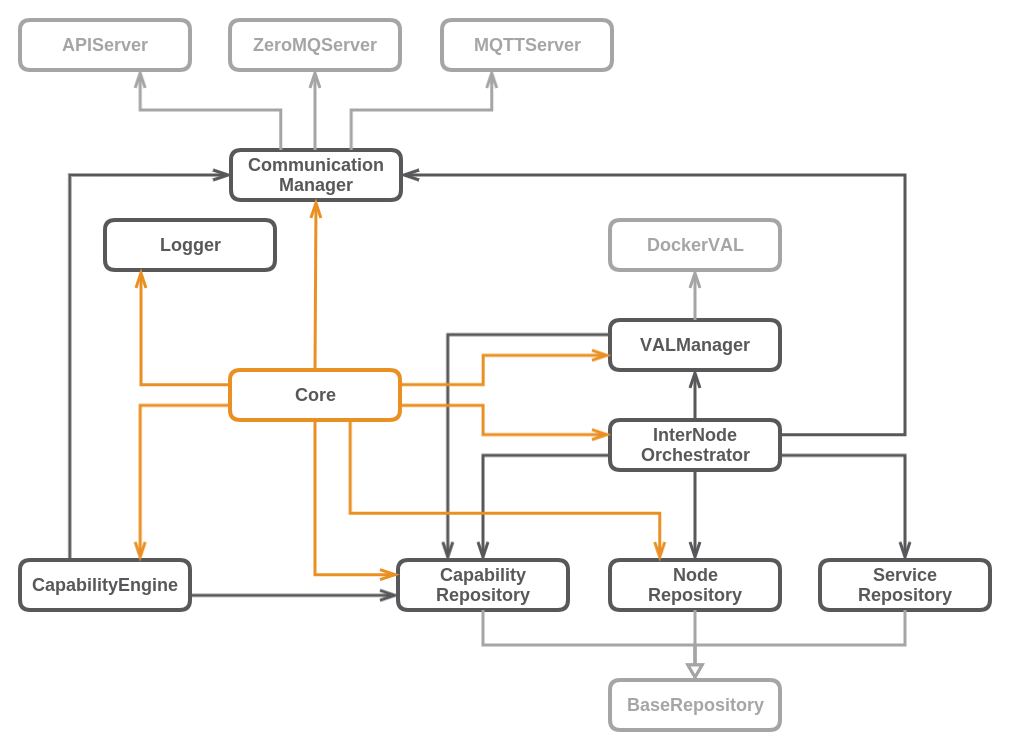
\includegraphics[width=\textwidth]{resources/images/class_diagram.png}
    \caption[Motey class diagram]{Motey class diagram}
    \label{fig:motey_class_diagram}
\end{figure}

Another example for that behavior is the \textit{VALManager}.
Also this class acts as a decorator and manages all virtualization plugins, in this case the \textit{DockerVAL}.
The repositories are a special case of the decorator pattern, because they covers the usage of the \textit{TinyDB} library, but they are also a centralized place for using them instead of all over in the engine.
The \textit{CapabilityEngine} and the \textit{InterNodeOrchestrator} are the only component that uses the \textit{CommunicationManger}.
The \textit{Core} also imports that class but only to start them.
Beside the \textit{Core} the \textit{InterNodeOrchestrator} is the central place in the app.
Each event will be executed in the layer.
Therefore most of the other components will be come together in this class.
In the following the separate layers are described in detail.


\subsection{Data layer}
\label{subsection:impl-data-layer}
As mentioned before TinyDB is used as the database engine of choice.
To abstract TinyDB from the rest of the source code, the repository pattern will be used.
Each content type has its own database and also a related repository.
All of them are inheriting from the \textit{BaseRepository}.
This repository is used to implement some default methods and will also create the database path in the constructor if it is necessary.
Beside that all of them are pretty similar implementation-wise.
They only differ in using different models and have some specific methods to be executed.
These models are used to represent the related \ac{JSON} objects.
Therefore each of them have a static transform method to convert \ac{JSON} objects to the related model.
The models folder also contains a file called \textit{schemas.py}.
This file contains the validation schemes for the different \ac{YAML} and \ac{JSON} objects that could be received by the nodes.
A library called \textit{jsonschema} is used to validate the objects based on such a schema.
An example for a schema is shown in listing \ref{code:capability-schema}.
\begin{listing}[H]
  \begin{minted}{python}
  capability_json_schema = {
      "type": "array",
      "items": {
          "type": "object",
          "properties": {
              "capability": {
                  "type": "string"
              },
              "capability_type": {
                  "type": "string"
              }
          },
          "required": ["capability", "capability_type"]
      }
  }
  \end{minted}
  \caption{Capability JSON validation schema}
  \label{code:capability-schema}
\end{listing}
The \textit{jsonschema} library allows to validate the type of an entry (line 2, 7 and 10) and also if the fields are required or optional (line 13).
This guarantees that only valid objects will be processed.

Another data layer component is the configuration reader.
This is implemented with the default Python \textit{configparser}.
The parsed configuration is only kept in memory.
The configuration file for the whole project is stored in the \textit{motey/configuration} folder and is called config.ini.
Listing \ref{code:config-ini} show the sample content of that file.
\begin{minted}{python}
[GENERAL]
app_name = Motey
pid = /var/run/motey.pid

[LOGGER]
name = Motey
log_path = /var/log/motey/
file_name = application.log

[WEBSERVER]
ip = 0.0.0.0
port = 5023

[MQTT]
ip = 172.18.0.3
port = 1883
keepalive = 60
username = neoklosch
password = neoklosch

[DATABASE]
path = /opt/Motey/motey/databases

[ZEROMQ]
capability_engine = 5090
capabilities_replier = 5091
deploy_image_replier = 5092
image_status_replier = 5093
image_terminate_replier = 5094
\end{minted}
\captionof{listing}{Example of the config.ini file\label{code:config-ini}}
\vspace{0.5cm}
Different sections can be separated by squared brackets like \textit{[GENERAL]} like on line 1.
The entries are simple key-value pairs.
Line 3 for example set the path to the used pid file.
The usage of the configreader is shown in listing \ref{code:configreader-example}.

\begin{listing}[H]
  \begin{minted}{python}
  from motey.configuration.configreader import config

  daemon = Daemonize(
      app=config['GENERAL']['app_name'],
      pid=config['GENERAL']['pid'],
      action=run_main_component
  )
  \end{minted}
  \caption{Example of the usage of the configreader}
  \label{code:configreader-example}
\end{listing}
The configuration object must be imported from the configreader module (see line 1) and can be used directly afterwards (line 4 and 5).
Due to the implementation of the import logic in Python, the containing script will be executed only once, regardless how many files import that module.

\subsection{Orchestration layer}
The so called InterNodeOrchestrator contains the main business logic of the application.
It is the connector between the communication layer or more specific between all inter-node and client communication endpoints and the \ac{VAL}.
The orchestrator uses the observer pattern to interact with the communication layer.
At the startup of the orchestrator it will subscribe to an observer for example for receiving a new service.
If a service event occurs, it will start the \textit{instantiate\_service} method.
This will be executed in a separate thread.
At first the service will be stored in the data layer.
The lifecycle will be changed to the \textit{instantiating} state.\newline

Afterwards the capabilities of each contained image has to be checked.
This is necessary to identify the node that is handling the image.\newline

There are three different possibilities:
\begin{enumerate}
  \item there are no capabilities located in the image, therefore the current node starts the image.
  \item there are capabilities and the current node is able to fulfill all of them. The same node is handling the image.
  \item there are capabilities but the current node is not able to fulfill one or multiple of them. Another node has to be search to manage the image.
\end{enumerate}
\bigskip

The capabilities of the current node are fetched via the \textit{CapabilityRepository}.
In each case the an image will always get an \ac{IP} address of the node that is handling them, even if it is the current node.
Later on the communication layer will deploy the image via an ZeroMQ connection.
This unifies the deployment process.
If the current node is not able to fulfill all required capabilities another node in the cluster will be searched to run the image.
Therefore the \textit{find\_node} method is going to be used.
This method will at first fetch all the known nodes from the \textit{NodeRepository}.\newline

Afterwards it will send out a \textit{capabilities request} again via the communication layer.
That is a ZeroMQ request-reply call between two nodes.
The targeted node sends back their capabilities.
They will be passed back to the orchestrator which compares them with the capabilities of the image.
If all of the are fulfilled then, this node becomes responsible for that image.
This means the \ac{IP} address of the node will be stored in the image.
If the node is not able to accomplish them, the next node is requested.
When non of the nodes suits, the state of the deployment will be marked as \textit{error} and cancelled at the same time.
Otherwise the deployment phase starts.
Each image will be passed via ZeroMQ call to the related \ac{IP} address to a deployment endpoint, which will then call the \textit{VALManager}.
The latter will then instantiate the image via the related \ac{VAL} plugin.
When all images finally started the state of the service will change to \textit{running} and the deployment successfully finished.\newline

The state of the service is also handled by the orchestrator.
It depends highly on the state of the images.
If at least only a single image is in a \textit{error} state, the whole service will be marked as erroneous.
This behaviour is similar for the other states.
Based on the \ac{MANO} service lifecycle the following states was created:\newline

\begin{itemize}
  \item \textbf{INITIAL} - The service is created, but no other action was performed so far.
  \item \textbf{INSTANTIATING} - The deployment phase was started, but is not done yet.
  \item \textbf{RUNNING} - All images are deployed and the service is running. Everything works normal.
  \item \textbf{STOPPING} - The termination phase was executed, but is not done yet.
  \item \textbf{TERMINATED} - All images are terminated. The service no longer exist.
  \item \textbf{ERROR} - An error occurred in one of the other states. A detailed description is stored in the service.
\end{itemize}
\bigskip

All of them are located in a model object called \textit{ServiceState}.

If a service state request is performed by the client, the request will then be received in the communication layer and passed over to the orchestrator.
Afterwards The \textit{get\_service\_status} method is executed which maps the states of the images to the service state.
Listing \ref{code:service-state-lifecycle} shows this method.

\begin{listing}[H]
  \begin{minted}{python}
  def get_service_status(self, service):
    image_status_list = []
    for image in service.images:
        image_status = self.communication_manager.request_image_status(image)
        image_status_list.append(image_status)

    if Image.ImageState.ERROR in image_status_list:
        service.state = Service.ServiceState.ERROR
        self.terminate_service(service=service)
    elif Image.ImageState.TERMINATED in image_status_list:
        service.state = Service.ServiceState.TERMINATED
        self.terminate_service(service=service)
    elif Image.ImageState.STOPPING in image_status_list:
        service.state = Service.ServiceState.STOPPING
        self.terminate_service(service=service)
    elif Image.ImageState.INSTANTIATING in image_status_list:
        service.state = Service.ServiceState.INSTANTIATING
    elif Image.ImageState.INITIAL in image_status_list:
        service.state = Service.ServiceState.INITIAL
    elif len(image_status_list) > 0 and image_status_list[1:] == image_status_list[:-1] and \
            image_status_list[0] == Image.ImageState.RUNNING:
        service.state = Service.ServiceState.RUNNING
    else:
        service.state = Service.ServiceState.ERROR

    self.service_repository.update(dict(service))
    return service.state
  \end{minted}
  \caption{The mapping of the service lifecycle state.}
  \label{code:service-state-lifecycle}
\end{listing}

Important in this method is that each status will again be requested via an ZeroMQ endpoint.
Also in this case a request-reply call between the nodes will be executed.
Line 4 show this request.
As all states are received and stored the mapping starts.
Line 10 up to 12 show the mapping of the \textit{terminated} state.
At first the list with all image states will be searched for this particular state.
If it is in the list, also the service will be marked as terminated.
To make sure that all the related service images are terminated, not only a single one, all the other images will be terminated as well.
Line 12 shows the termination of the service.
This behavior is also implemented for the \textit{error} and \textit{stopping} state.
All the other states are mapped directly to the service.
Finally the new state will be stored in the \textit{ServiceRepository} and the state returned (line 26 and 27).\newline

The termination of a service is pretty similar to the creation beside the fact that there is no capability comparison and node retrieval.
The image termination command will directly passed over to the related node.
Also this method will be executed in a separate thread to not block the main thread.

\subsection{Communication layer}
\label{subsection:implementation-communication-layer}
As mentioned in section \ref{subsection:CommunicationLayer} the communication layer is splitted up into three different components as is decorated by an extra layer called \textit{CommunicationManager}.
The important implementation details of all of them will be described in this subsection.
All the necessary communication components are located in the \textit{motey/communication} folder.

\paragraph{APIServer} This server is responsible for the \ac{REST} \ac{API}.
Therefore the Flask server will be instantiated and configured in the constructor of the wrapper class.
The server will be executed in a separate thread due to the nature of a webserver to block the main thread because the it will run endless to receive all incoming requests.
If it would not be implemented with a thread only the Flask server would be started and the following code would be blocked.
Furthermore Flask has to be configured to accept cross-site requests, by disabling the \textit{same origin policy} with a \textit{\ac{CORS}} library.
This behavior is a development only feature and it is strictly recommend to deactivate it in production mode.
By deactivating it the server is vulnerable for \ac{CSRF} and clickjacking attacks.
In the development phase cross-site requests should be allowed to make it easier to communicate between a web client and the \ac{REST} \ac{API}.
In addition all the configured \ac{API} will be initialized.
As mentioned before these routes can be implemented as Flask Blueprints.
All routes are located in the \textit{motey/communication/api\_routes} directory.\newline

There are four different routes:
\begin{itemize}
  \item The \textbf{Capabilities} Blueprint which is used to send the capabilities of the node, add new capabilities or to remove them.
  The \ac{HTTP} verb \textit{GET} is used to deliver all existing capabilities.
  If a request is received, the \textit{CapabilityRepository} will be used to fetch all capabilities and then they will be converted to a JSON string afterwards.
  The \ac{HTTP} verb \textit{PUT} will add new entries to the repository.
  After the \ac{JSON} request will be received, the content will be parsed and validated with the corresponding \ac{JSON} schema.
  If it is not valid or the content type of the request is not \textit{application/json} a \ac{HTTP} status code 400 is returned.
  Otherwise the capabilities will be added via the \textit{CapabilityRepository} to the database.
  This will end up in the \ac{HTTP} status code 201.
  The same logic will be used for the \textit{DELETE} request.
  \item The second endpoint is implemented as the \textbf{Nodes} Blueprint.
  The only functionality is to respond with all stored nodes as \ac{JSON}.
  This is used for testing purposes and could also be helpful for maintaining the cluster.
  \item To get some information about the node health status the \textbf{NodeStatus} Blueprint was created.
  It respond with some hardware information like the current \ac{CPU} or memory usage.
  This is also useful for maintaining the nodes.
  \item The last Blueprint implementation is the \textbf{Service} endpoint.
  It is used to get a \ac{JSON} list with all stored services via the \ac{HTTP} \textit{GET} verb and also to deploy and remove services.
  Therefore the \textit{POST} or \textit{DELETE} verb is used.
  Both implementations are pretty similar.
  Also in this case the provided \ac{YAML} file will be validated.
  If it is valid the parsed service will be handed over to the orchestration layer and a 201 will be returned to the client.
  If something went wrong a 400 will be returned.
\end{itemize}

\paragraph{MQTTServer}
The purpose of using \ac{MQTT} in the Motey engine is the node discovery.
Section \ref{subsection:CommunicationLayer} describes the basic idea of it.
To implement the logic the node must have knowledge about the \ac{IP} and port of the \ac{MQTT} broker as well as the authentication credentials if they are required.
They can be configured via the global configuration file.
As all the other classes, the \textit{MQTTServer} is a wrapper class for the Python \ac{MQTT} library.
In the constructor the routes will be defined as well as some callbacks and the client will be configured.
The \textit{start} method connects the client to the broker and execute the request loop.
That is pretty similar to the implementation of the \textit{APIServer}.
Therefore the \ac{MQTT} client has to be executed in a separate thread too.

\begin{figure}[H]
    \centering
    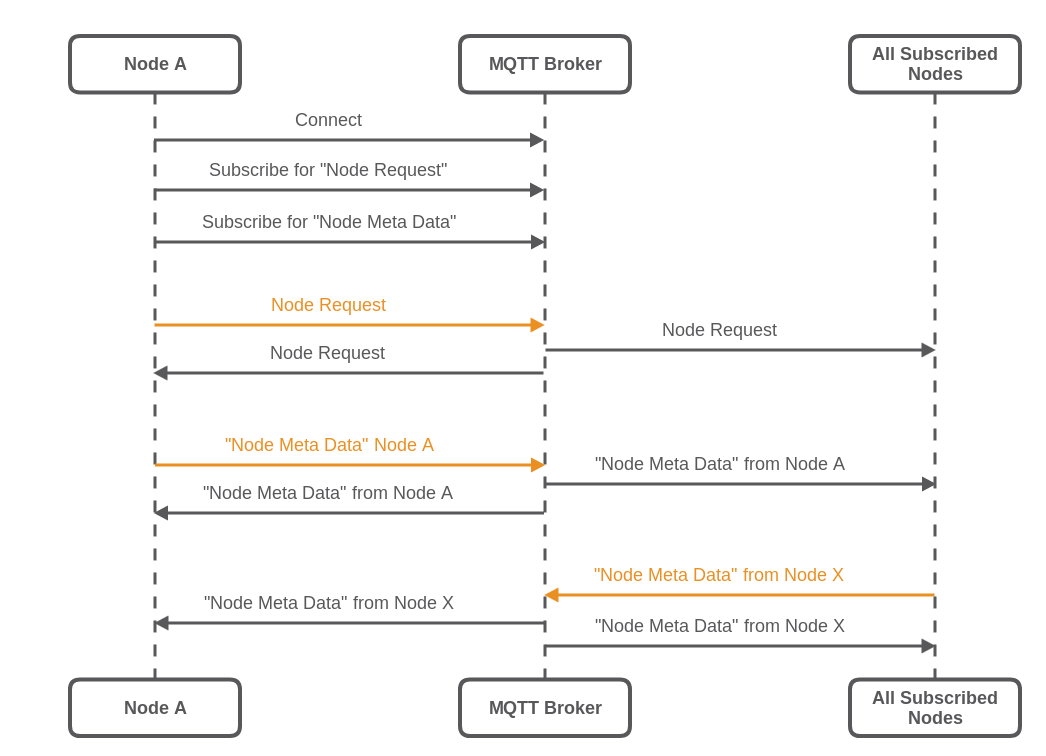
\includegraphics[width=\textwidth]{resources/images/node_discovery.png}
    \caption[Node discovery sequence diagram]{Node discovery sequence diagram}
    \label{fig:node_discovery_squ_dia}
\end{figure}

Figure \ref{fig:node_discovery_squ_dia} shows how the node discovery will be implemented.
Important aspect is that the sender node is also part of the subscribed nodes.
This means after the \textit{connection} to the broker is established and the client is subscribed to the topics, each \textit{Node Request} will also be received by the sender himself.
Benefit out of it, is that beside the fact that a new registered node gets all meta information from all other nodes, also these nodes get the meta information of the new node.
In this way each node has knowledge of all the other nodes and can keep track of them.\newline

This is also the reason why the \textit{"Node Meta Data" from Node A} and \textit{"Node Meta Data" from Node X} are duplicated in figure \ref{fig:node_discovery_squ_dia}.
Beside that the procedure is straight forward: At first one node send out a \textit{Node Request}.
Each subscribed node will get it and send out a response with the \textit{Node Meta Data} to all the other nodes via the broker.
The \textit{after\_connect} handler will be used to send out the \textit{Node Request} after a new nodes is successfully subscribed to the broker.
Before a node disconnects, a \textit{Remove Node} request will be send out, that will inform each node that a specific node will be disappear.
All the nodes react to this by removing the meta data about this node from the database.

\paragraph{ZeroMQServer}
Section \ref{section:ZeroMQ} and \ref{subsection:CommunicationLayer} gave a detailed overview about ZeroMQ and how does it work.
Now the concrete implementation will be discussed.
The wrapper class \textit{ZeroMQServer} binds multiple sockets to the related ports.
There are four sockets binded for the direct node-to-node communication via \ac{TCP} and one port to connect third party applications to the Motey engine.
The latter is used to add or remove capabilities on a node.
ZeroMQ provides an \ac{IPC} protocol for such a use case.
The ZeroMQServer will bind a socket with the Publish-Subscribe pattern that allows multiple publisher to connect to the endpoint.
Two important aspects have to be considered by using the Publish-Subscribe pattern in ZeroMQ.
As in \ac{MQTT} each subscription has to be done to a topic.
Listing \ref{code:ZeroMQ-pub-sub} show the subscription for the \textit{capabilityevent} at line 3.
This also means that it is possible to send multiple different events to a single socket endpoint.
In Motey this feature is not used yet, but nevertheless it is necessary to subscribe to a topic because of the implementation specification of ZeroMQ.
Without that, the subscriber will receive nothing.

\begin{listing}[H]
  \begin{minted}{python}
  def start(self):
    self.capabilities_subscriber.bind('ipc://*:%s' % config['ZEROMQ']['capability_engine'])
    self.capabilities_subscriber.setsockopt_string(zmq.SUBSCRIBE, 'capabilityevent')
    # [...]

  def __run_capabilities_subscriber_thread(self):
    while not self.stopped:
        result = self.capabilities_subscriber.recv_string()
        topic, output = result.split('#', 1)
        self.capability_event_stream.on_next(output)
  \end{minted}
  \caption{Example of the usage of the configreader}
  \label{code:ZeroMQ-pub-sub}
\end{listing}

The second important aspect is at line 9.
An incoming message has always been parsed for a delimiter.
The reason for that is, that the topic, in this case \textit{capabilityevent} have to be prepend to the message followed by the delimiter.
Listing \ref{code:ZeroMQ-capability-event-msg} show such a message.
\begin{listing}[H]
  \begin{minted}{bash}
  capabilityevent#{'capability': 'zigbee', 'capability_type': 'hardware'}
  \end{minted}
  \caption{Example ZeroMQ capability event message}
  \label{code:ZeroMQ-capability-event-msg}
\end{listing}
Therefore the topics and the delimiter has to be removed before the message can be parsed.\newline

The other four sockets are implemented with the Request-Reply pattern and are used to:
\begin{itemize}
  \item reply to a capability request.
  This is used by the \textit{InterNodeOrchestrator} to get the capabilities of other nodes.
  The result is send as a \ac{JSON} string.
  If there are no capabilities an empty \ac{JSON} array will be send.
  \item deploy images is also used by the \textit{InterNodeOrchestrator} to deploy a single image to another node.
  The image model will be transformed to a \ac{JSON} object and send over as a string and vice versa and passed over to the \textit{VALManager} if received.
  \item return the status of an image. This is also used by the \textit{InterNodeOrchestrator} when the state of a service should be fetched. To current state of an image will be detected by the virtualization engine. Afterwards it will transformed to a unified image state. Finally the InterNodeOrchestrator maps the state of all images to the service state.
  \item terminate an existing image instance.
  Only the image id has to be send to perform that action.
  The \textit{VALManager} will handle the termination of the instance.
\end{itemize}
\bigskip

Important aspect while using the Request-Reply pattern, there can only be one connection established at the same time.
In addition a reply must send by the consumer after a request was receive.
As long as there was no message send back, the connection will be blocked and the consumer can not receive any new messages.\newline

As discussed by the other servers, also this one have to be executed in threads.
Difference here is that each socket has its own thread.
This is necessary because each connection waits for a request and has its own request loop.
Therefore each loop would block the main thread.

\paragraph{CommunicationManager}
Finally the \textit{CommunicationManager} is used to decorate the servers from the rest of the source code.
This is helpful for decoupling the components as well as replace or add a new communication component.
Beside that the manager simply forward the methods to the specific server.
It is also used as a central place to start and stop all servers.


\subsection{Capability management}
Similar to the InterNodeOrchestrator the \textit{CapabilityEngine} is used as a connector between the communication layer and the in this case CapabilityRepository.
Therefore the main components of the capability management are the CapabilityEngine and the \textit{ZeroMQServer}.
The latter was extensively described in the previous section and is mainly used to receive new capabilities or to remove them after a request via one of the two ZeroMQ endpoints.
The CapabilityEngine on the other side has two subscriptions to the observer located in the ZeroMQServer.
These subscriptions reacts to add and remove requests of any external application.
Due to the fact that the endpoints are implemented via the ZeroMQ \ac{IPC} protocol only application that are located on the node can interact with the CapabilityEngine.
After a new add service request was received the \ac{JSON} data will be parsed, validated and transformed to the capability model and afterwards stored via the \textit{CapabilityRepository} to the database.
The Removal of an entry is pretty similar.
The received \ac{JSON} data will be again validate with the \textit{capability\_json\_schema} from the schemes model.


\subsection{User interface}
The whole Motey \ac{GUI} is located in a separate folder called \textit{webclient}.
Due to the fact that the \ac{GUI} is only for demonstration purposes, it should not be part of the main engine.
Vue.js the used web framework is pretty lightweight, therefore only two files are necessary to execute the client.
The \textit{index.html} file contains the skeleton of the page.
In addition to that the \textit{main.js} file that is located in the \textit{js} folder contains the business logic of the page.
Figure \ref{fig:motey_gui_screenshot} shows the final \ac{GUI}.
\begin{figure}[H]
    \centering
    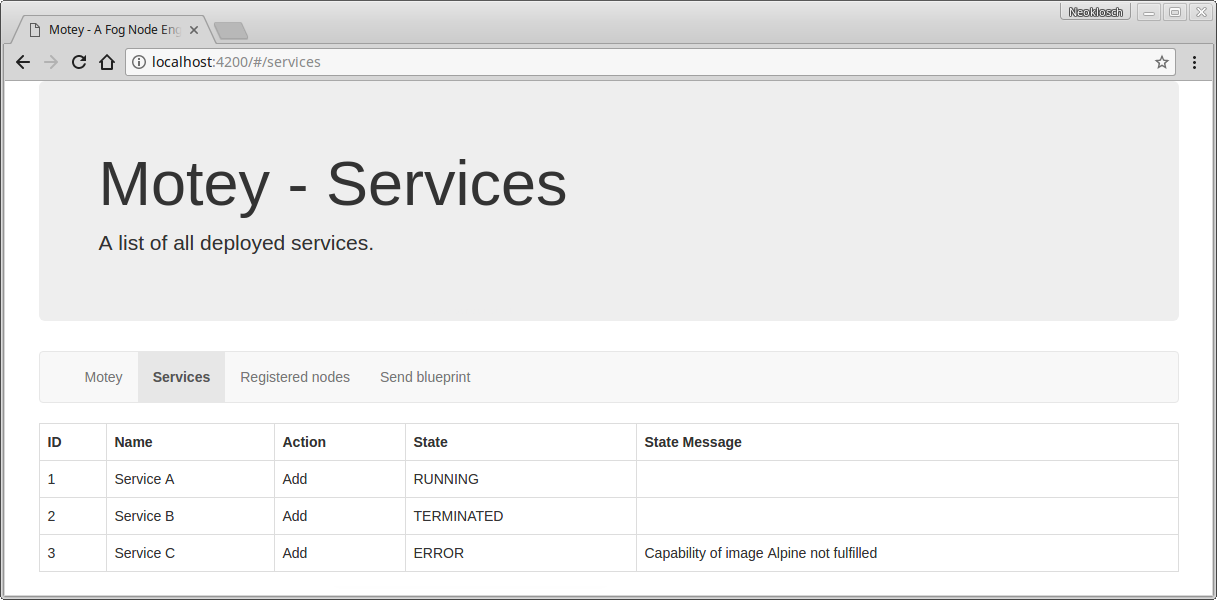
\includegraphics[width=\textwidth]{resources/images/motey_gui_screenshot.png}
    \caption[Screenshot of the Motey \ac{GUI}]{Screenshot of the Motey \ac{GUI}}
    \label{fig:motey_gui_screenshot}
\end{figure}
The header is fixed and only contains the name of the engine and a short description of the page content.
Below them the navigation bar located.
As in the mockup four different pages are available.
The first called \textit{Motey} has a very short introduction into the web client.
The second and also the selected one in the screenshot shows a list with all deployed services.
\textit{Registered nodes} will show a list with all discovered nodes, again in a table.
Finally the \textit{Send blueprint} contains a textarea to put in the \ac{YAML} service description and a button to send the data.\newline

The \textit{index.html} file contains also the files for the bootstrap and Vue.js libraries.
They are loaded from a \ac{CDN} provider to speed up the loading time.
This is possible because if the user already visited a page that uses the same \ac{CDN} provider and the same libraries, they will be cached in the browser internal cache.
If the user then visits another site that try to load the files, they will be taken from the cache instead of requested again.
This increases the page loading speed as well as reduces the traffic.
Another benefit is that the files does not have to be stored on the server.\newline

Beyond that the \textit{main.js} file initializes the routes to handle the navigation bar redirects.
Each route has an own controller similar to the Blueprint concept of the Flask server.
The \textit{NodesListing} and \textit{ServiceListing} controllers mainly fetches the \ac{JSON} data from the \ac{REST} \ac{API} and map them to the related template in the \ac{HTML} file.
The \textit{BlueprintTemplate} controller get the data from the textarea and send them over to the \ac{API}.
Finally the \textit{Content-Type} of the request will be set to \textit{application/x-yaml} as specified in the server endpoint.
As defined before, there is no user authentication or other access control mechanisms due to the fact that this \ac{GUI} is exclusively made for testing purposes.

\subsection{Deployment and Continuous Integration}
Travis CI as the tool of choice for the \ac{CI} uses a \textit{.travis.yml} configuration file.
The content of the file is shown in listing \ref{code:travis_config}.

\begin{listing}[H]
  \begin{minted}{yaml}
  sudo: true
  services: docker
  language: python
  os: linux
  cache: pip
  python:
    - "3.6"

  install: "pip install -r motey-docker-image/requirements.txt"

  script:
    - pycodestyle --ignore=E241,E501 motey/
    - pycodestyle --ignore=E241,E501 samples/
    - python3 -m unittest tests/capabilityengine/test_* tests/communication/test_* tests/models/test_* tests/orchestrator/test_* tests/repositories/test_* tests/utils/test_* tests/val/test_*

  after_success:
    - if [[ "$TRAVIS_BRANCH" = "master" ]]; then
      docker build -t neoklosch/motey motey-docker-image;
      docker login -u="$DOCKER_USERNAME" -p="$DOCKER_PASSWORD";
      docker push neoklosch/motey;
      fi
  \end{minted}
  \caption{Travis CI configuration file}
  \label{code:travis_config}
\end{listing}

There are some important parts in it.
At first the script need root privileges to build and upload Docker images.
Line 1 add this privilege and in line 2 the Docker service is requested.
The programming language the application to build is written in, is declared in line 3, in this case python.
Line 6 and 7 defines the python version to use.
There could be multiple, but due to the fact that the script should only be build one Docker image and should only upload them once, only one python version can be used.
Otherwise multiple python version would be executed and after each successfully build version an container would be build and uploaded.\newline

Line 9 defines the installation script.
This will executed after the virtual environment are created by Travis CI.
In this case the python requirements will be installed.
Line 11 up to 14 are used to test the source code.
A code style check is performed in line 12 and 13.
It will check to code against the \ac{PEP} 8 standard\footnote{\url{https://www.python.org/dev/peps/pep-0008}}, which is be used by several other libraries like the pretty famous Django project{\interfootnotelinepenalty10000 \footnote{\url{https://docs.djangoproject.com/en/dev/internals/contributing/writing-code/coding-style}}}.
After that all the related unit tests will be executed.
If there is an error during the execution of the \textit{script} block, the whole build process will be stopped and marked as error.
The current state can be view in Travis CI at \url{https://travis-ci.org/Neoklosch/Motey} and also in the readme of the project at \url{https://github.com/Neoklosch/Motey} or \url{http://motey.readthedocs.io/en/latest}.\newline

The \textit{after\_success} block is used to create and upload the Docker image.
Beside that the install routine and also the \ac{CI} commands are similar.
The image will only be executed if it is a master branch build (see line 17).
This is reasonable because a development branch build can be unstable and should not be used to create an official Docker image.
Line 18 will build the image and line 19 uploads it.
Two environment variables are used here, because to upload an image, the username and the password of the Docker Hub account has to be passed.
Due to the fact that this file is under public version control, this sensible information should not be commited.
Therefore preconfigured login credentials are used.
Finally the Docker image will be pushed in line 20.\newline

In the root folder of the Motey project there are two Docker image directories.
The first one can be used to create and upload a normal Docker image and it is called \textit{motey-docker-image}.
That folder is also used in the \textit{after\_success} block.
The second folder can be used to build and upload a specific Raspberry Pi Docker image.
Both scripts are slightly different, because a Raspberry Pi is using a \ac{CPU} with an ARM architecture.
Therefore Docker images that should support ARM \acp{CPU} must have specific dependencies and has to be build differently.
To build an image, a so called \textit{Dockerfile} has to be created.
The Dockerfile for the Raspberry Pi image is different to the one for the nomal image, because it load a Raspbian base image instead of an Ubuntu image like the normal file will do.
Also the setup script is slightly different, because Raspbian sometimes need other dependencies or has different preinstalled tools.
Listing \ref{code:motey_dockerfile} shows the Dockerfile for the normal Motey build.

\begin{listing}[H]
  \begin{minted}{dockerfile}
  FROM ubuntu:xenial

  MAINTAINER Neoklosch version: 0.0.1

  ADD ./setup.sh /tmp/setup.sh
  ADD ./requirements.txt /tmp/requirements.txt
  RUN /bin/bash /tmp/setup.sh

  EXPOSE 5023 5091 5092 5094 5094 1883

  CMD ["motey", "start"]
  \end{minted}
  \caption{Dockerfile to create the Motey Docker image}
  \label{code:motey_dockerfile}
\end{listing}

The \textit{FROM} command at line 1 defines the base image.
In this case it is an \textit{Ubuntu} image in version 16.04 also called Xenial Xerus, which has a long-time support and is a pretty stable version.
The \textit{ADD} command is used to add external files to the Docker container to be executed later or make them available in the image.
The script adds a \textit{setup.sh} file that is executed in line 7.
This file uses the \textit{requirements.txt} file, that is also added.
Additional the ports in line 9 are exposed, which means they are provided to the Docker engine as used by the container.
There is no automatic mapping between the host and the guest system ports, but they can be mapped much faster due to the \textit{EXPOSE} command.
Finally the \textit{CMD} command will execute a specific shell command, in this case the \textit{motey start} command.\newline

This command is available after Motey was installed by the \textit{setup.py} file in the root folder.
To install Motey, only two build steps has to be executed, that are shown in listing \ref{code:motey_setup}.

\begin{listing}[H]
  \begin{minted}{bash}
  python3 setup.py build
  python3 setup.py install
  \end{minted}
  \caption{Motey setup procedure}
  \label{code:motey_setup}
\end{listing}

When the installation routine is done, the \textit{motey} command becomes available globally.
The usage of the command line tool was shown in \ref{library:daemonize}.
Beside the installation via the setup script, Motey can also be added as a Docker container named \textit{neoklosch/motey}.
This method is preferred to make the first steps with Motey, because it is more isolated from the host system, easier to use, to remove and to update.

\section{Code Verification}
\label{section:code-verification}
Code verification is a quite important technique in every development project.
There are several possibilities to check and verify the integrity of the created source code.
Two of them are used in this project.
The style check is used to ensure the compliance with the code style guidelines and the unit tests are used to verify the correctness of the code and the outcome of the functions itself.
As the guidelines the pretty famous \ac{PEP} 8 style guide\footnote{\url{https://www.python.org/dev/peps/pep-0008}} is used.
\ac{PEP} 8 is used in the Python standard library code and is well established in the community.
A standardized code style is recommended in team projects as well as in open source projects.
But also in private project a commitment to a specific style can be helpful to make the project easier to maintain.
The code in general becomes more readable, more understandable and the amount of errors can be decreased.
Due to the fact that overall code is read more often than it is written, other people will be satisfied by having a common understanding of the "grammar" of the code to be used.
As the tool of choice the library \textit{pycodestyle} will be used.
The style check is part of the \ac{CI} pipeline and the concrete implementation was shown in listing \ref{code:travis_config}.
If there is any style check violation, the \ac{CI} build process will fail and the new Docker image will not be uploaded.

\begin{listing}[H]
  \begin{minted}{bash}
  $ pycodestyle --ignore=E241,E501 motey/
  motey/di/app_module.py:48:38: E128 continuation line under-indented for visual indent
  motey/di/app_module.py:49:38: E128 continuation line under-indented for visual indent
  motey/di/app_module.py:50:38: E128 continuation line under-indented for visual indent
  motey/di/app_module.py:51:38: E128 continuation line under-indented for visual indent
  motey/di/app_module.py:52:38: E128 continuation line under-indented for visual indent
  motey/di/app_module.py:53:38: E128 continuation line under-indented for visual indent
  motey/di/app_module.py:54:38: E128 continuation line under-indented for visual indent
  motey/configuration/configreader.py:6:66: E703 statement ends with a semicolon

  The command "pycodestyle --ignore=E241,E501 motey/" exited with 1.

  $ pycodestyle --ignore=E241,E501 samples/

  The command "pycodestyle --ignore=E241,E501 samples/" exited with 0.
  \end{minted}
  \caption[Sample output of the style check validation from the Travis CI build process number 148]{Sample output of the style check validation from the Travis CI build process number 148\autocite{Travis:Build:148}}
  \label{code:style_check_validation}
\end{listing}

Listing \ref{code:style_check_validation} shows an example output of the Travis \ac{CI} build process.
The first style check call fails due to multiple validations, but the second one exited successfully.\newline

The second verification is are the unit tests.
A unit test is as the name implies a software test method which tests each component of an application.
This method is a white box test, because the source code of the well known and only the results are tested.
Each component should be tested as isolated as possible by invoking only one or a couple of methods from a unit and the result should be verified automatically and compared with an expected result.\autocite[cf.][p. 320]{Olan:2003:UTT}
All the used objects in a class should be as independent from each other as possible.
To ensure this, the objects have to be mocked by a mocking framework.
The python unit test framework has a build-in mocking framework since version 3.
A mock is a fake objects that acts as a dummy for the class to be tested.
To decouple the dependencies and to increase the testability and more specific to make used object easier mockable, the \ac{DI} pattern is used.
Each injected object can be easily mocked outside of the class.
Due to the fact that Python allows to modify each class member at any time, \ac{DI} is not really necessary, but it helps to make it clearer to understand and the code more readable and maintainable.\newline

The advantages of unit tests in general are that problems can be easier localized and much faster detected.
If an error occurs during unit testing a former well working code, it is obvious that the last code changes are the reason for the error.
This benefit is also helpful to reduce the fear of refactoring or extend code parts.
Even pretty old parts of an application can be modified without the risk of any major problems.
When the unit test are part of the \ac{CI}, each build will be checked.
This reduces the risk of the deployment of faulty code.
And finally unit tests can be a good starting point for new team members, because it helps to understand the functionality of a class.
An unit test can acts as some kind of documentation.

\begin{listing}[H]
  \begin{minted}{python}
  class TestServiceRepository(unittest.TestCase):
    @classmethod
    def setUp(self):
        self.text_service_id = uuid.uuid4().hex
        self.test_service = {'id': self.text_service_id, 'service_name': 'test service name', 'images': ['test image']}
        service_repository.config = {'DATABASE': {'path': '/tmp/testpath'}}
        service_repository.BaseRepository = mock.Mock(service_repository.BaseRepository)
        service_repository.TinyDB = mock.Mock(TinyDB)
        service_repository.Query = mock.Mock(Query)
        self.test_service_repository = service_repository.ServiceRepository()

    def test_has_entry(self):
        self.test_service_repository.db.search = mock.MagicMock(return_value=[1, 2])

        result = self.test_service_repository.has(service_id=self.test_service['id'])

        self.assertTrue(self.test_service_repository.db.search.called)
        self.assertTrue(result)
  \end{minted}
  \caption{Extract from the Motey unit test of the ServiceRepository}
  \label{code:sample_unit_test}
\end{listing}

The downsides are that unit tests are coded.
This means also unit tests can have errors and they have to be maintained if the source code of the main project is changed.
Furthermore poorly written unit tests or tests that are written unmotivated can end up in a wrong feeling of safeness.
Some error case could not be caught and the submitted code is still faulty.
Additionally the test setup is not a realistic environment.
Integration test are in general more accurate in terms of the human behavior.
They test complete workflows and not only single components or functions.
Also the dependencies between the component and the interaction between them can be tested much better with integration test.
In many projects the most critical part of unit tests are, that they take time.
For each written component, the related tests take a significant time to be developed.
In a real life project this could be unacceptable even if it is important to have them.\newline

Listing \ref{code:sample_unit_test} shows an extract from the \textit{ServiceRepository} unit test.
The test starts with a \textit{setUp} method (line 3) that is executed before each test.
In this case some static variables will be created (line 4 - 6) and the internally used libraries are mocked (line 7 - 9).
Finally the \textit{ServiceRepository} itself will be created.
The \textit{test\_has\_entry} method is one of multiple tests.
This method checks if a value exists in the database.
Therefore the result of the database search method is mocked (line 13) and the \textit{has} command is executed (line 15).
Finally the results of the method are checked.
At first the script tests if a specific method is called, in this case the \textit{search} method of the database (line 17).
Afterwards the result of the \textit{ServiceRepository} \textit{has} method is checked (line 18).
If everything went fine, the test will execute with a status 0 as shown in listing \ref{code:style_check_validation}.

Unit testing in general can be realized in two different ways.
The first possibility is to write the tests after the coding of the component is done.
This is the standard way in many projects these days.
The advantage is that the code is done and normally no big changes comes after that.
This means also changes on the test suite are seldom.

The second possibility is the \ac{TDD}, that is related to the test-first programming concept of the extreme programming development.
In this development methodology the tests are written before the implementation of a class is created.
This helps to plan the architecture of a class and catch edge cases before the implementation is done.
\ac{TDD} is an iterative process where at first the test is written, then the test will be executed and must fail, afterwards the code is written and the tests should be executed again, but this time successfully.
Finally the process can be repeated for example if the code has to be refactored or extended.
Especially in an extreme programming environment \ac{TDD} in combination with pair programming and code reviews are reasonable.\newline

Motey was created with the "normal" unit testing approach, due to the fact that it was a one man project with rapidly changing requirements and an explorative approach to create the prototype.
Nevertheless both methods ends up in a well tested code base and an assured code stability.
